 This clusters job is to make sure that the user sees what is going on. It includes all scenes and menus, as well as displayers for the game players and status information.

\begin{itemize}
  \item{\textbf{PLAYER\_DISPLAYER}: This class displays the player on the map and prints the amount of tickets left. \texttt{PLAYER\_DISPLAYER} knows this information because of the client-supplier relationship with class \texttt{PLAYER}.}
  \item{\textbf{GAME\_SCENE}: Contains all the drawables of the current game scene and displays them.}
\end{itemize}

\begin{figure}[h]
\centerline{\hbox{  
  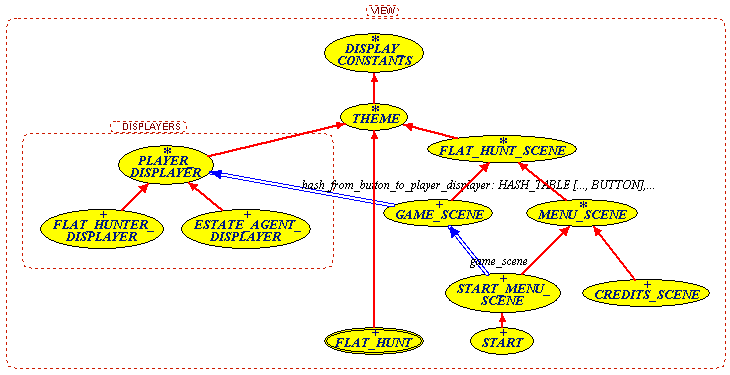
\includegraphics[width=135mm]{view}
  }}
\caption{Diagram of the View Cluster}
\label{viewdiagram}
\end{figure}
